\documentclass[a4paper,landscape]{article}
\usepackage{pdfpages}

\usepackage[margin=1cm]{geometry}

\usepackage{eso-pic}
\usepackage{mdframed}
\usepackage{tikz}

\begin{document}
\thispagestyle{empty}
\begin{tikzpicture}
  
  % \node[draw=none,fill=none] (main) 
  %   at (0,0){
  %     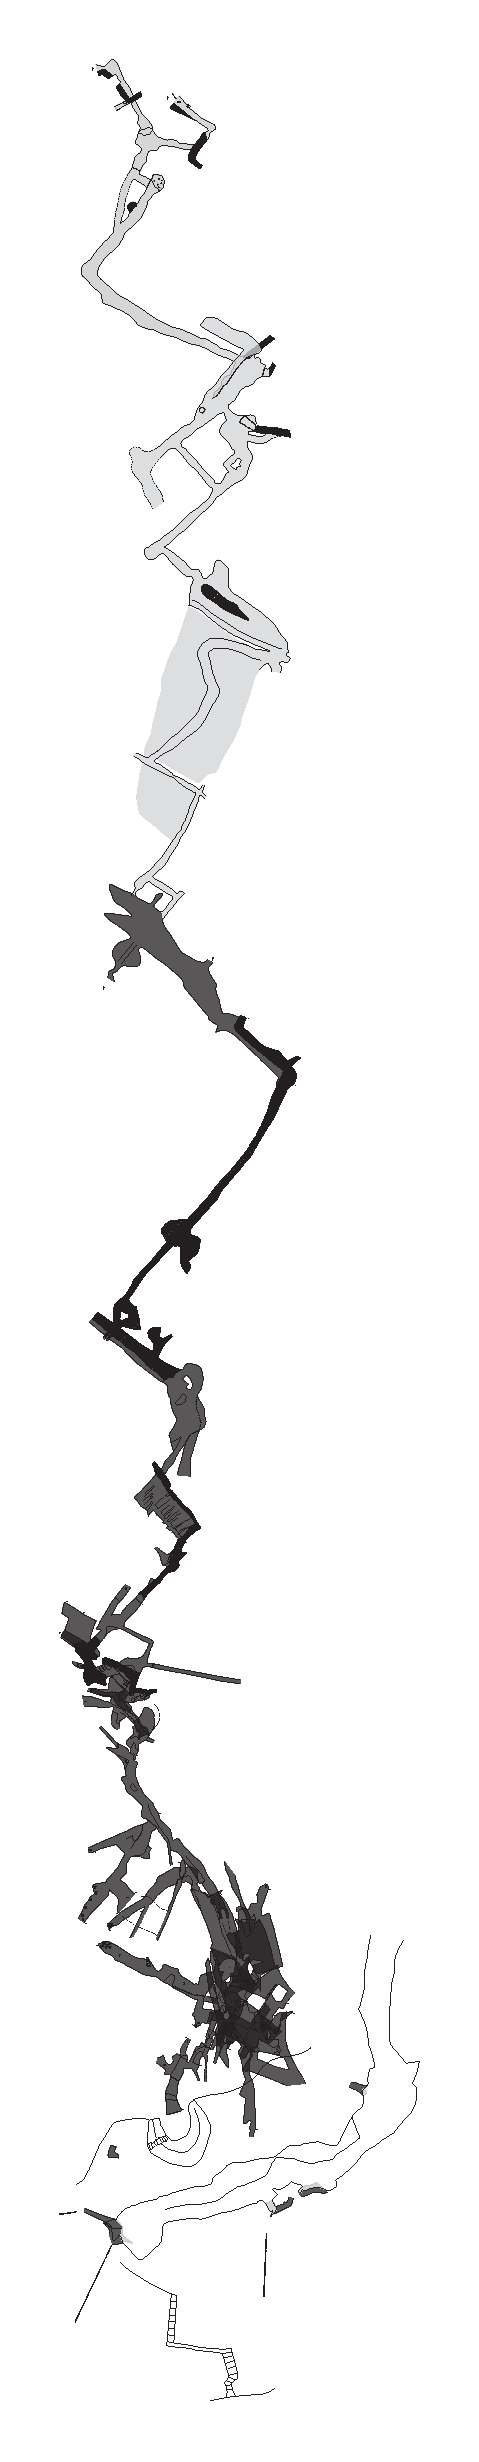
\includegraphics[height=0.98\textheight,keepaspectratio]{../../out/outline-plan.pdf}
  %   };
  \node[draw=red,fill=none,
    anchor=north west
  ] at (0,0) [right] {
    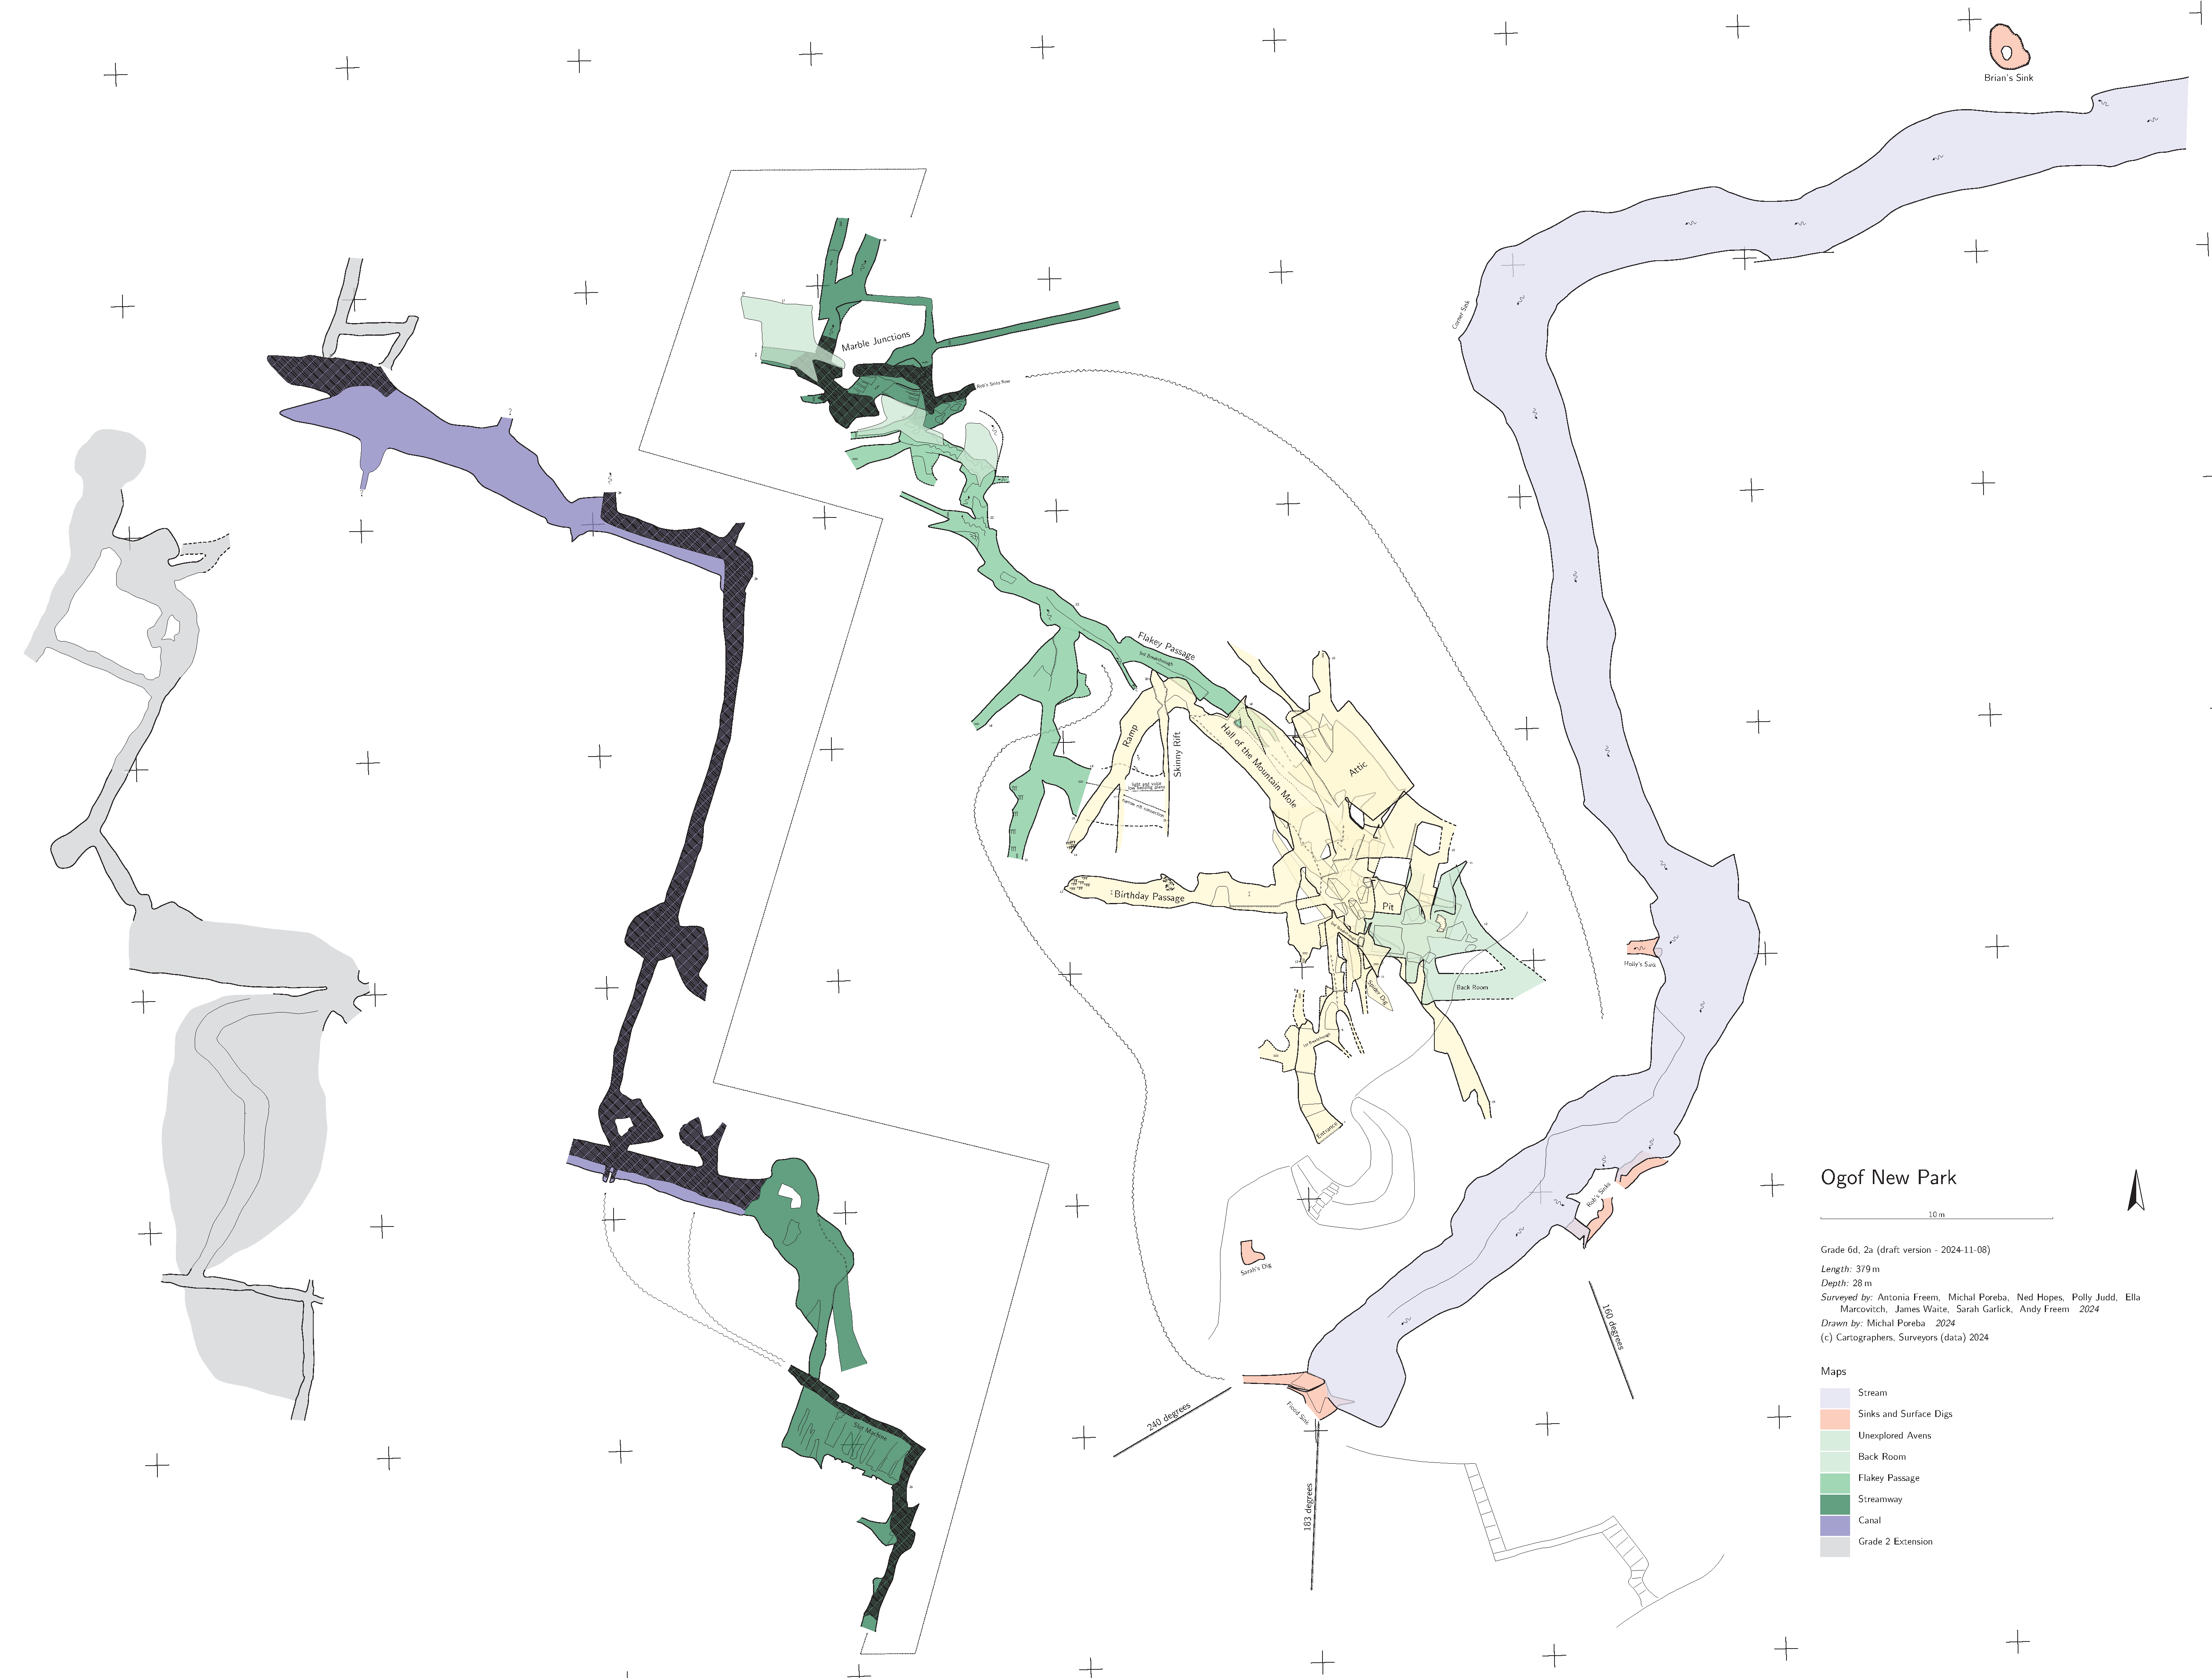
\includegraphics[trim={0 0 0 0}, clip, width=0.96\textwidth,keepaspectratio]{../../out/print-straight.pdf}
  };
  
  % \node[
  %   draw=none,fill=gray!20,text width=10cm,
  %   align=center,
  %   font=\bfseries\fontsize{24}{28}\selectfont,
  %   anchor=south west
  % ] 
  %   at (0,0) {
  %     Ogof Park Newydd / New Park Cave
  % };

  %\def\marginsize{1cm} 

  % Top Left
  %\draw[draw=black] (current page.north west) ++ (0,0) rectangle ++ (1cm,-1cm); 

  % Top Right
  %\draw[draw=black] (current page.north east) ++ (-\marginsize,-\marginsize) rectangle ++ (-1cm,-1cm);

  % Bottom Left
  %\draw[draw=black] (current page.south west) ++ (\marginsize,\marginsize) rectangle ++ (1cm,1cm);

  % Bottom Right
  %\draw[draw=black] (current page.south east) ++ (-\marginsize,\marginsize) rectangle ++ (-1cm,1cm);


  \end{tikzpicture}

\end{document}